\subsection{Kinect and fusionTrac 500 hand-eye calibration setup}

The \cref{fig:kinect_handeye_calibration_setup} shows the hand-eye calibration setup for Kinect with chessboard. Over 40 independent robot poses $\matr{M}$ were defined for hand-eye calibration. The robot drives to each of the defined positions where an image was taken using the Kinect camera. One should make sure that the chessboard is completely visible in the camera image. The pose of the chessboard in camera coordinates $\matr{N}$ is determined for each position by using the pose estimation algorithm very similar to camera extrinsic calibration. 30 poses were used for hand-eye calibration and rest 10 poses (which were not part of hand-eye calibration) were used for error estimation to avoid overfitting.

\begin{figure}[hbt!]
	\centering
	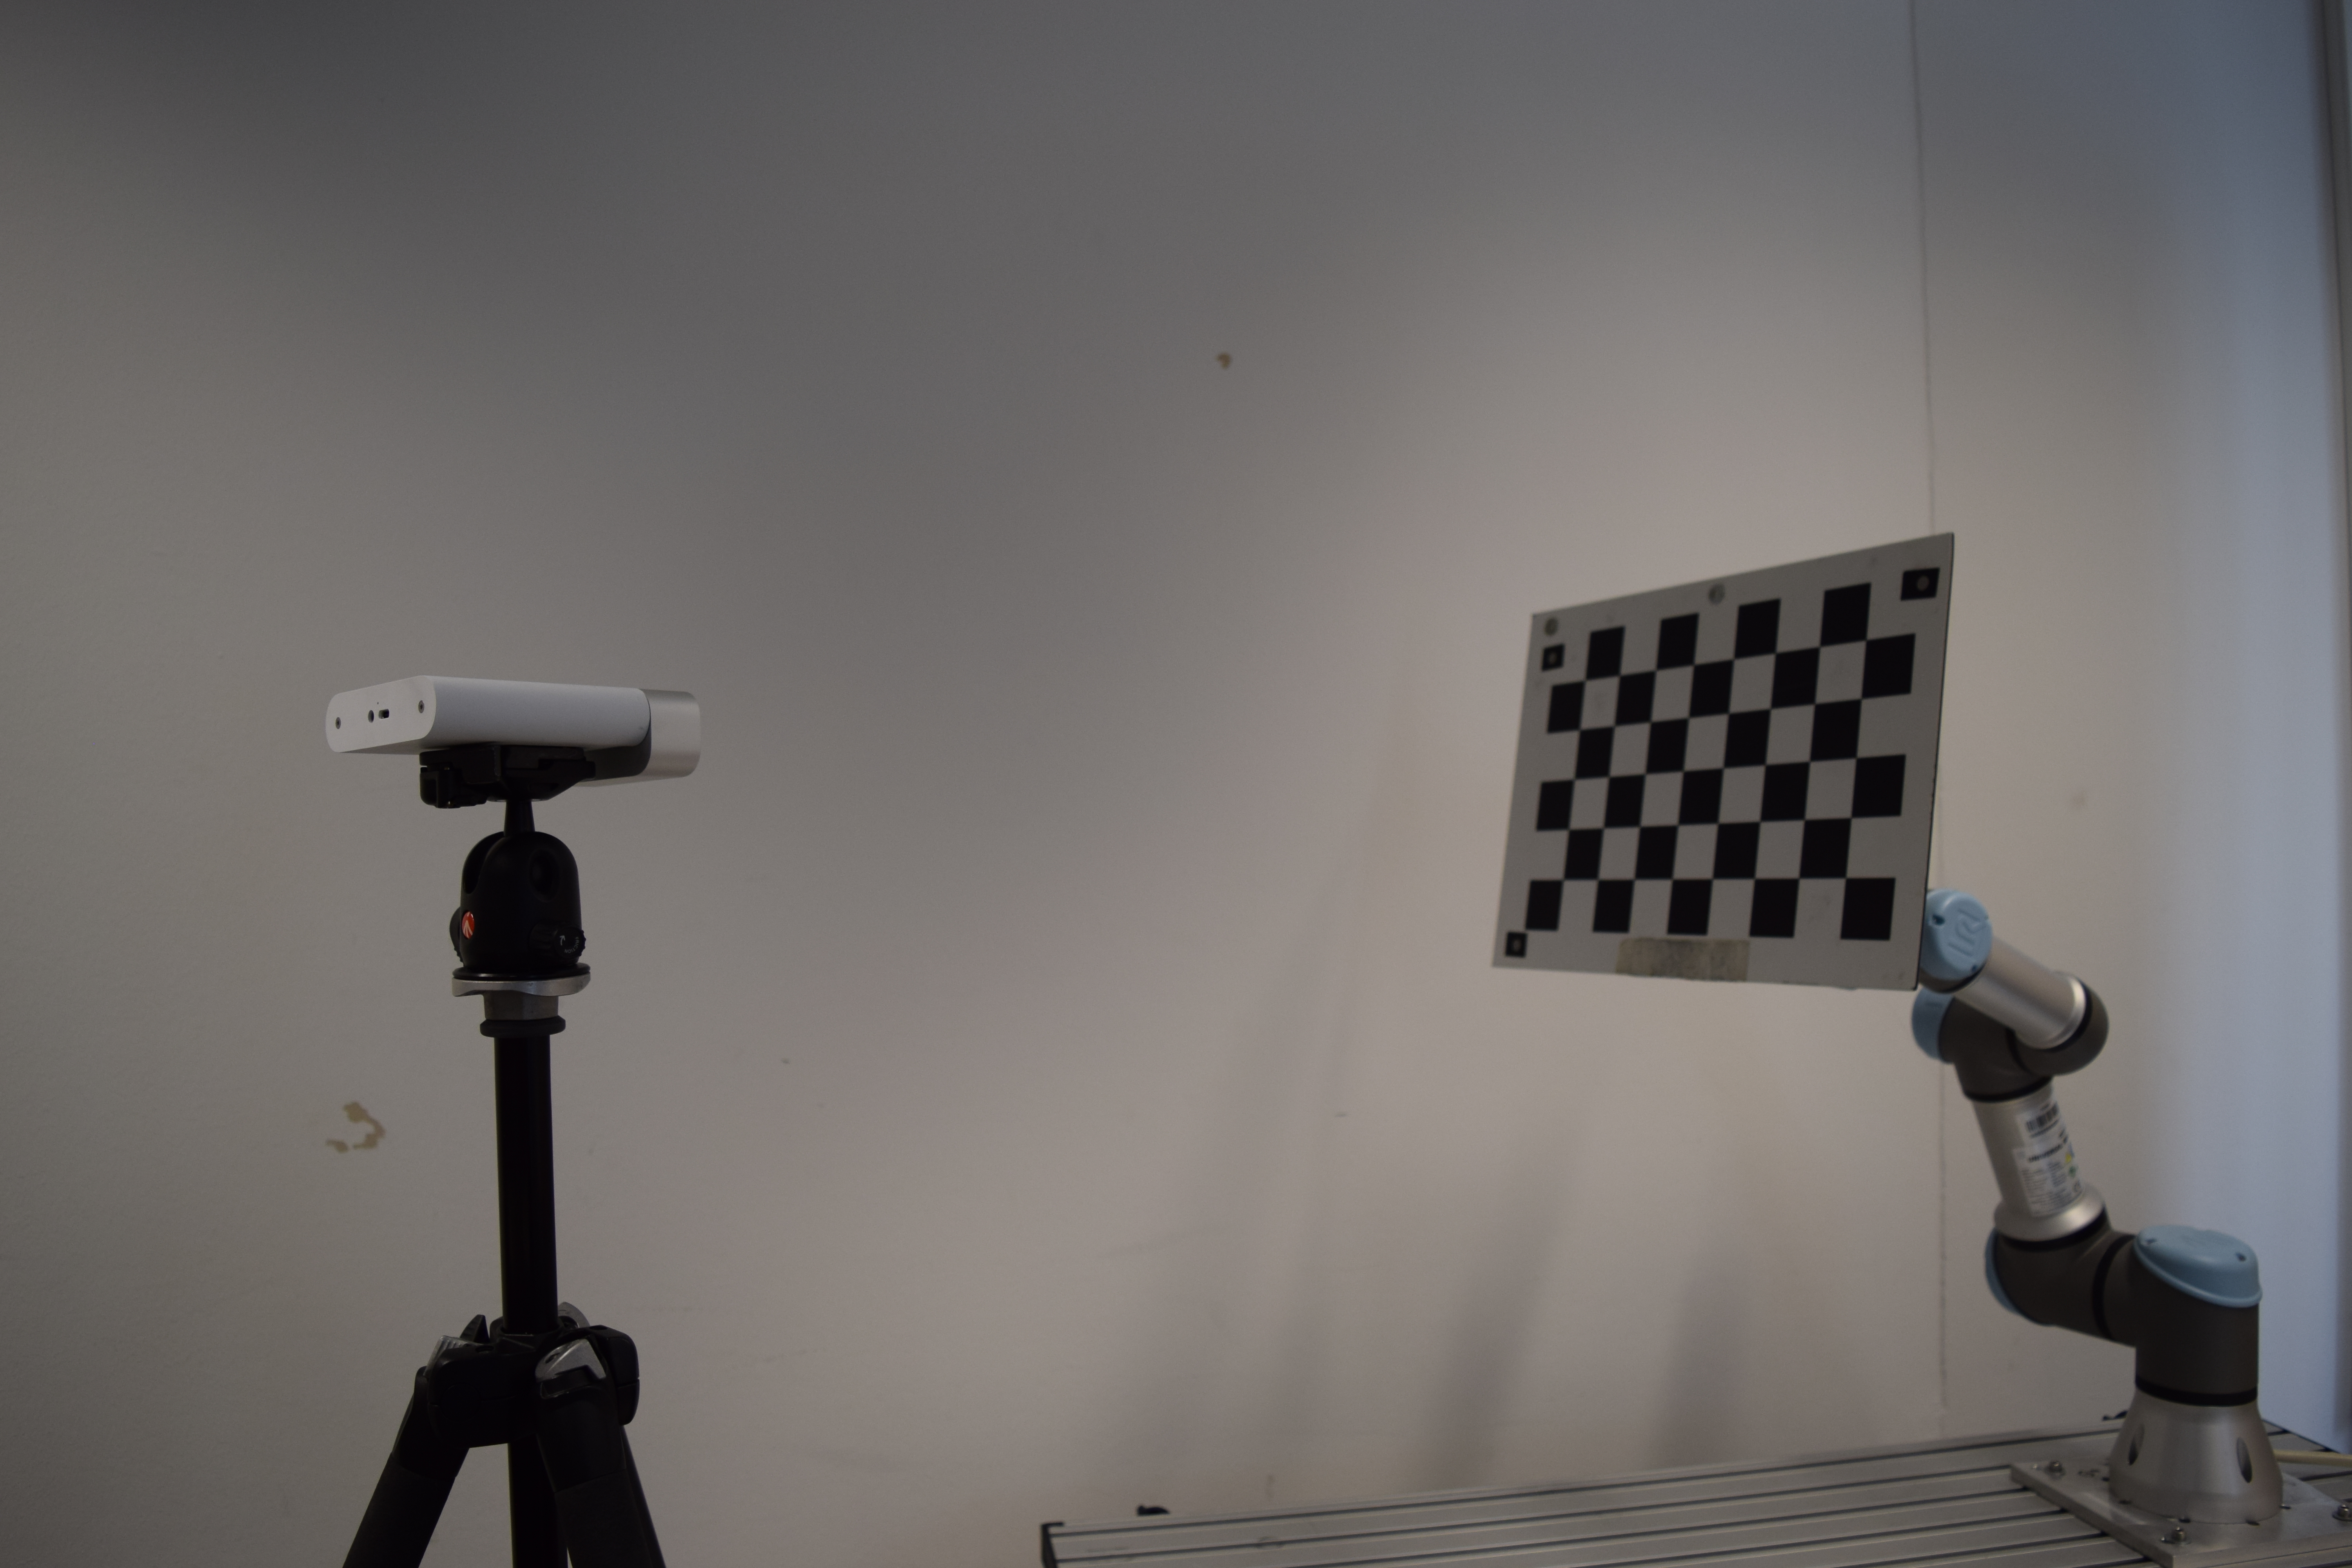
\includegraphics[width=\linewidth]{handeye_kinect.jpg}
	\caption{Kinect camera hand-eye calibration setup.} 
	\label{fig:kinect_handeye_calibration_setup}
\end{figure}

Same strategy goes for the fusionTrac 500 camera also with only exception that reflective marker has been used instead of chessboard as shown in the \cref{fig:handeye_fusionTrac}.\\

\begin{figure}[hbt!]
	\centering
	\begin{subfigure}{0.49\textwidth}
		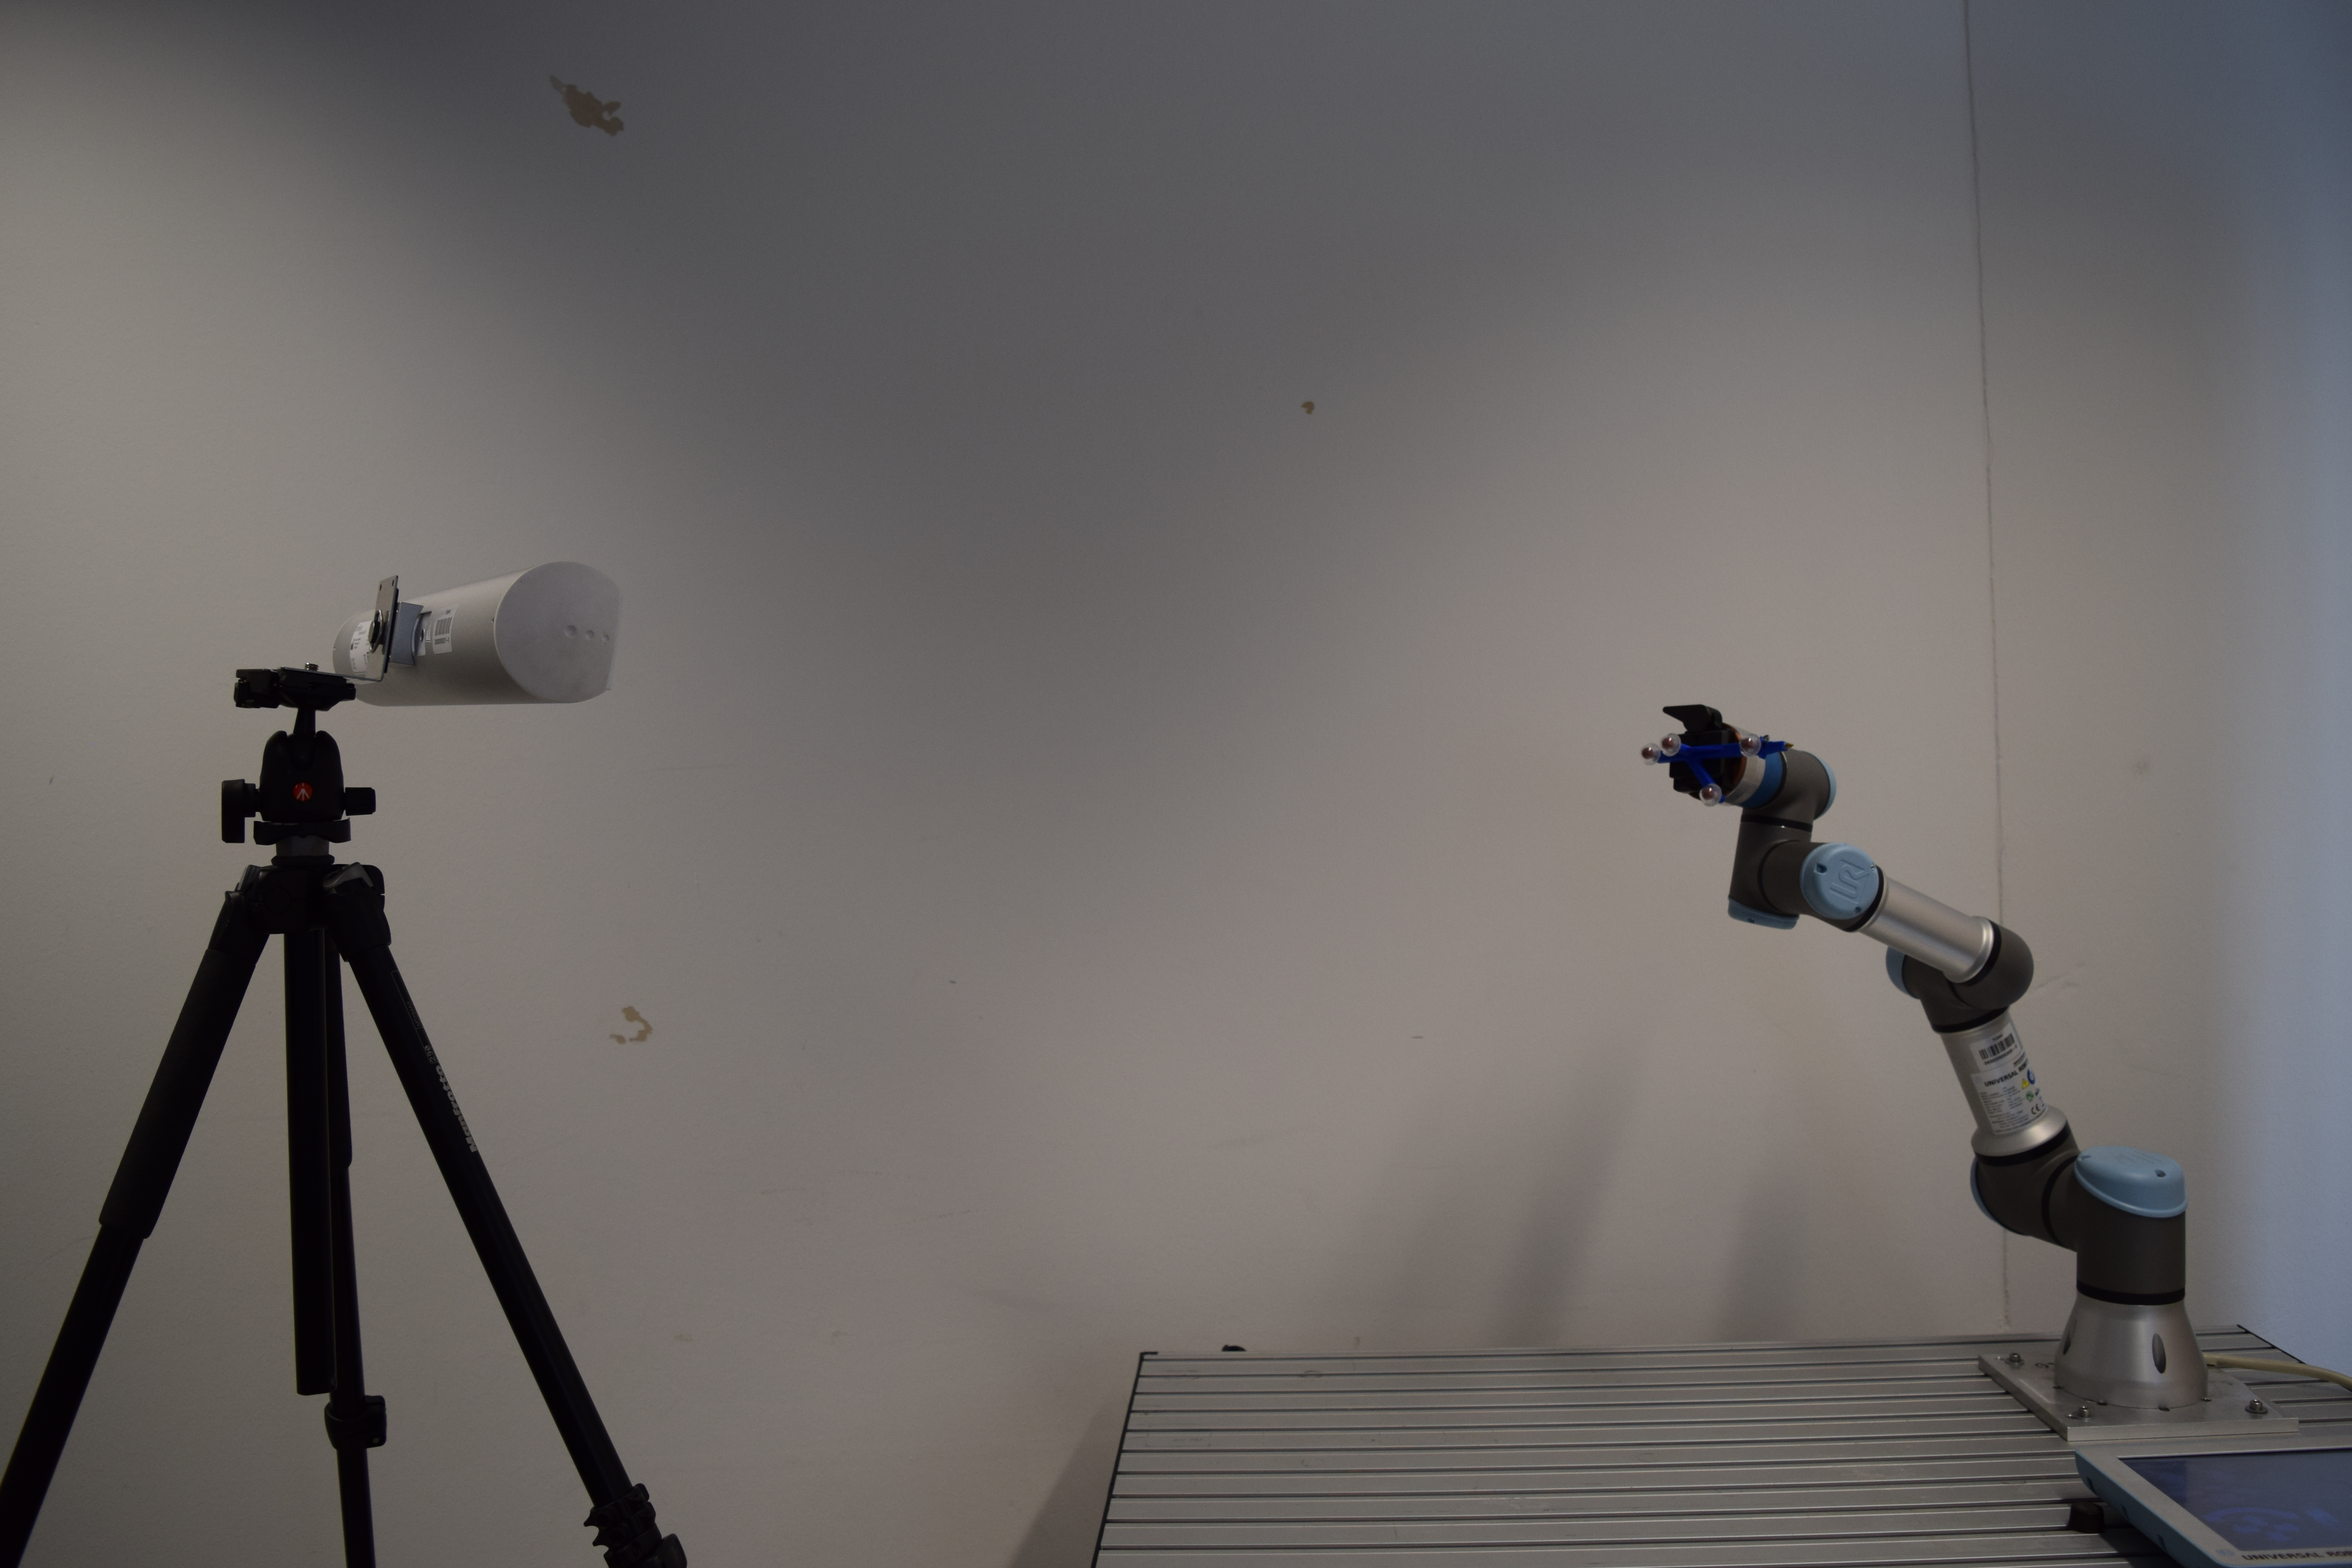
\includegraphics[width=\textwidth]{handeye_fusionTrac.jpg}	
	\end{subfigure}
	\hfill
	\begin{subfigure}{0.49\textwidth}
		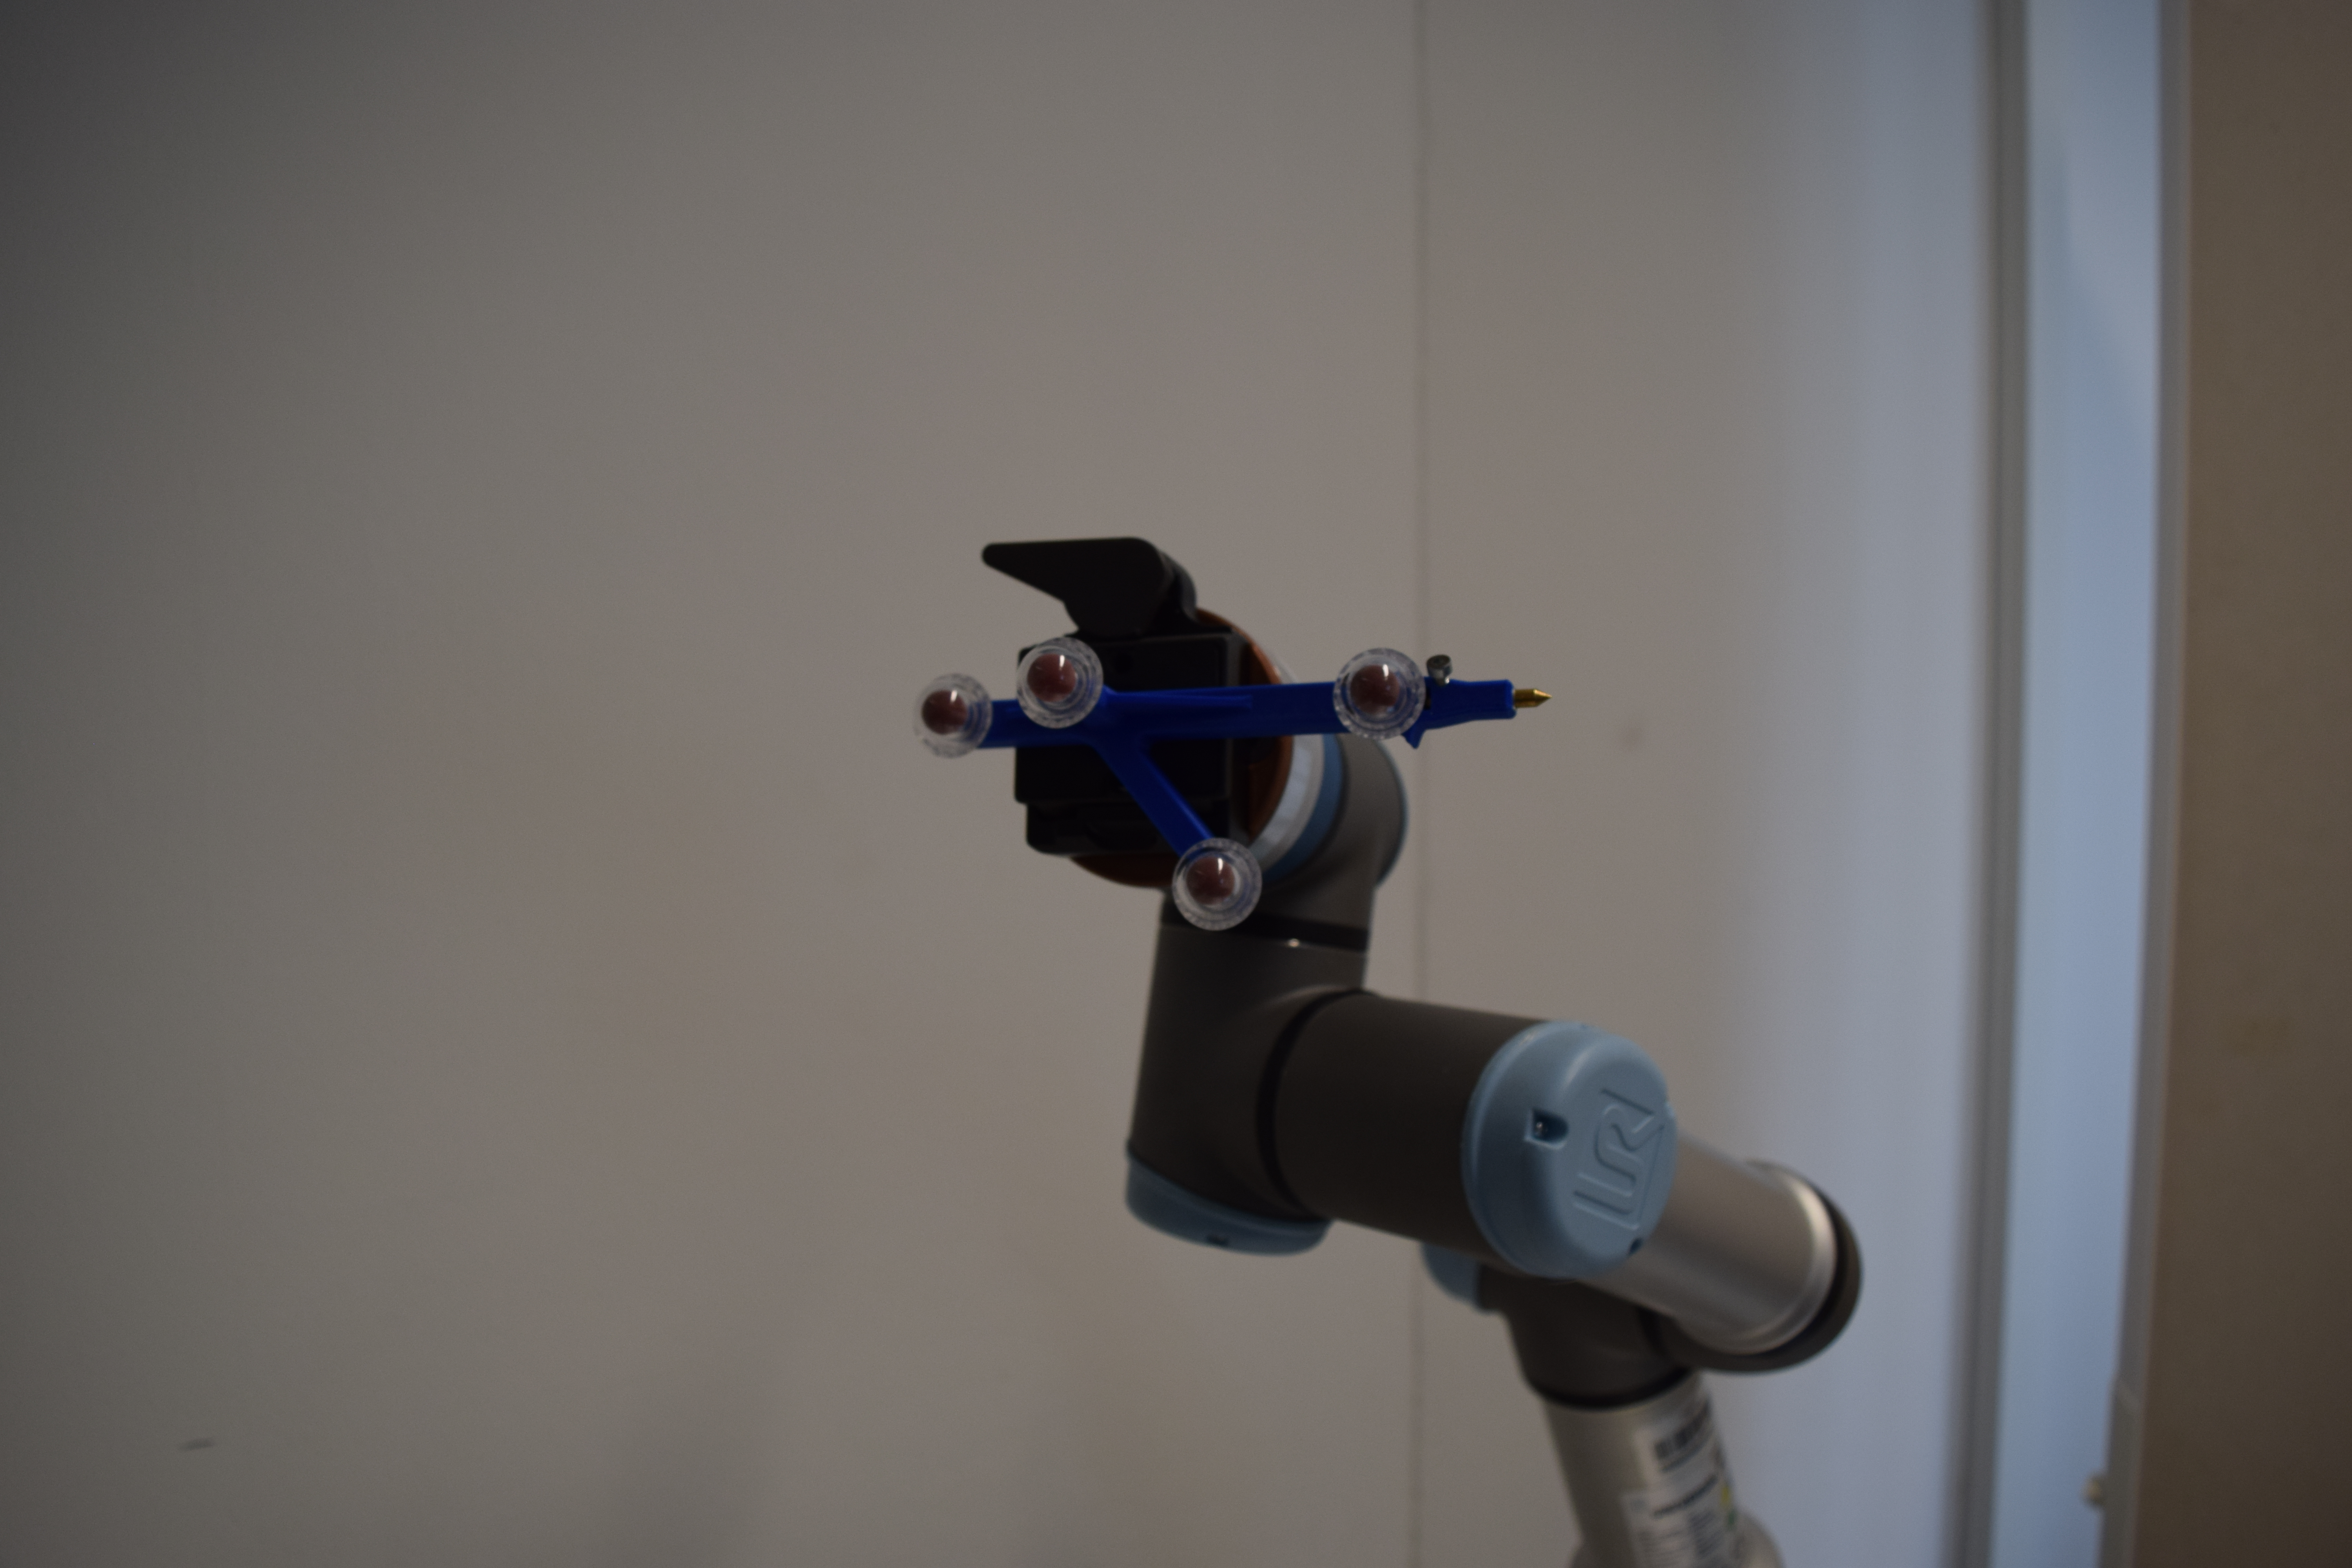
\includegraphics[width=\textwidth]{handeye_fusionTrac_2.jpg}	
	\end{subfigure}
	\caption{fusionTrac 500 camera hand-eye calibration setup.} 
	\label{fig:handeye_fusionTrac}
\end{figure} 